\documentclass[12pt,letterpaper]{article}

\newcommand\hwnumber{6}
\usepackage{fullpage}
\usepackage[top=2cm, bottom=4.5cm, left=2.5cm, right=2.5cm]{geometry}
\usepackage{amsmath,amsthm,amsfonts,amssymb,amscd}
\usepackage{lastpage}
\usepackage{enumerate}
\usepackage{fancyhdr}
\usepackage{mathrsfs}
\usepackage{xcolor}
\usepackage{graphicx}
\usepackage{listings}
\usepackage{hyperref}
\usepackage{enumitem}


\hypersetup{%
  colorlinks=true,
  linkcolor=blue,
  linkbordercolor={0 0 1}
}
% Reduce whitespace around figures
\setlength\intextsep{0pt}
 
 \newcommand{\twolines}{\vspace{5em}}
 \newcommand{\smallspace}{\vspace{12em}}
 \newcommand{\bigspace}{\vspace{60em}}
 
\renewcommand\lstlistingname{Algorithm}
\renewcommand\lstlistlistingname{Algorithms}
\def\lstlistingautorefname{Alg.}

\lstdefinestyle{Python}{
    language        = Python,
    frame           = lines, 
    basicstyle      = \footnotesize,
    keywordstyle    = \color{blue},
    stringstyle     = \color{green},
    commentstyle    = \color{red}\ttfamily
}

\setlength{\parindent}{0.0in}
\setlength{\parskip}{0.05in}
\setlist{leftmargin=2.5mm}

% Edit these as appropriate
\newcommand\course{CMPUT 397}


\pagestyle{fancyplain}
\headheight 35pt

\chead{\textbf{\Large Worksheet \hwnumber}}
\rhead{\course \\ \today}
\lfoot{}
\cfoot{}
\rfoot{\small\thepage}
\headsep 1.5em


\begin{document}

\begin{enumerate}
  %\item (\textit{Exercise 5.2 S\&B}) Suppose every-visit MC was used instead of 
first-visit MC on the blackjack task. Would you expect the results to be very
different? Why or why not?

%%%ANSWER%%%%
% The state depends on three variables, 
% 1) player's current sum
% 2) dealer's card
% 3) whether the player holds a usable ace
% this implies that the same state will not be visited more than
% once in an episode and first-visit will be the same as every-visit MC.

	%\item (\textit{Exercise 5.3 S\&B}) What is the backup diagram for Monte Carlo 
estimation of $q_\pi$?

	\item (\textit{Exercise 5.4 S\&B}) The pseudocode for \textit{Monte Carlo ES} is 
inefficient because, for each state-action pair, it maintains a list of all 
returns and repeatedly calculates their mean. How can we modify the algorithm
to have incremental updates for each state-action pair?
\begin{figure}[h!]
  \center
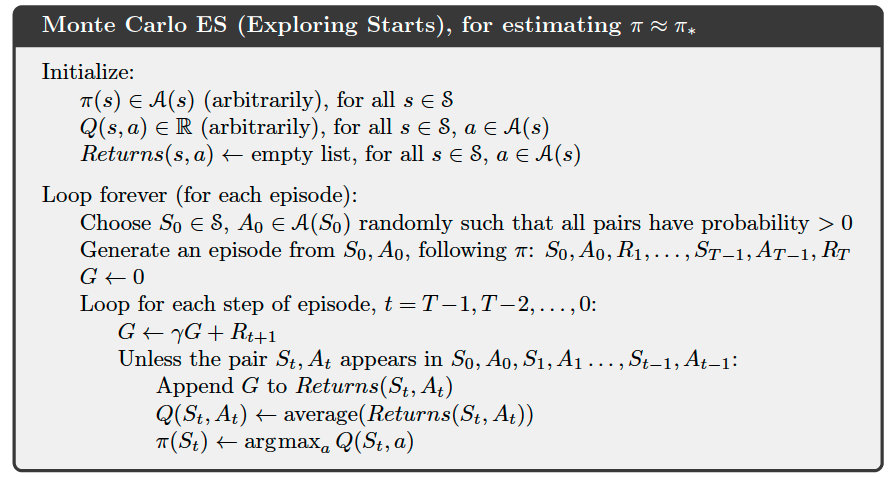
\includegraphics[width=0.8\linewidth]{figures/mc_es_pseudocode.png}
\end{figure}
	\item (\textit{Exercise 5.5 S\&B}) Consider an MDP with a single nonterminal state $s$ and
a single action that transitions back to $s$ with 
probability $p$ and transitions to the terminal state with probability $1-p$.
Let the rewards be $+1$ on all transitions, and let $\gamma=1$. Suppose
you observe one episode that lasts 10 steps, with return of 10. What
is the (every-visit) Monte-carlo estimator of the value of the nonterminal state $s$?
\begin{figure}[h!]
  \center
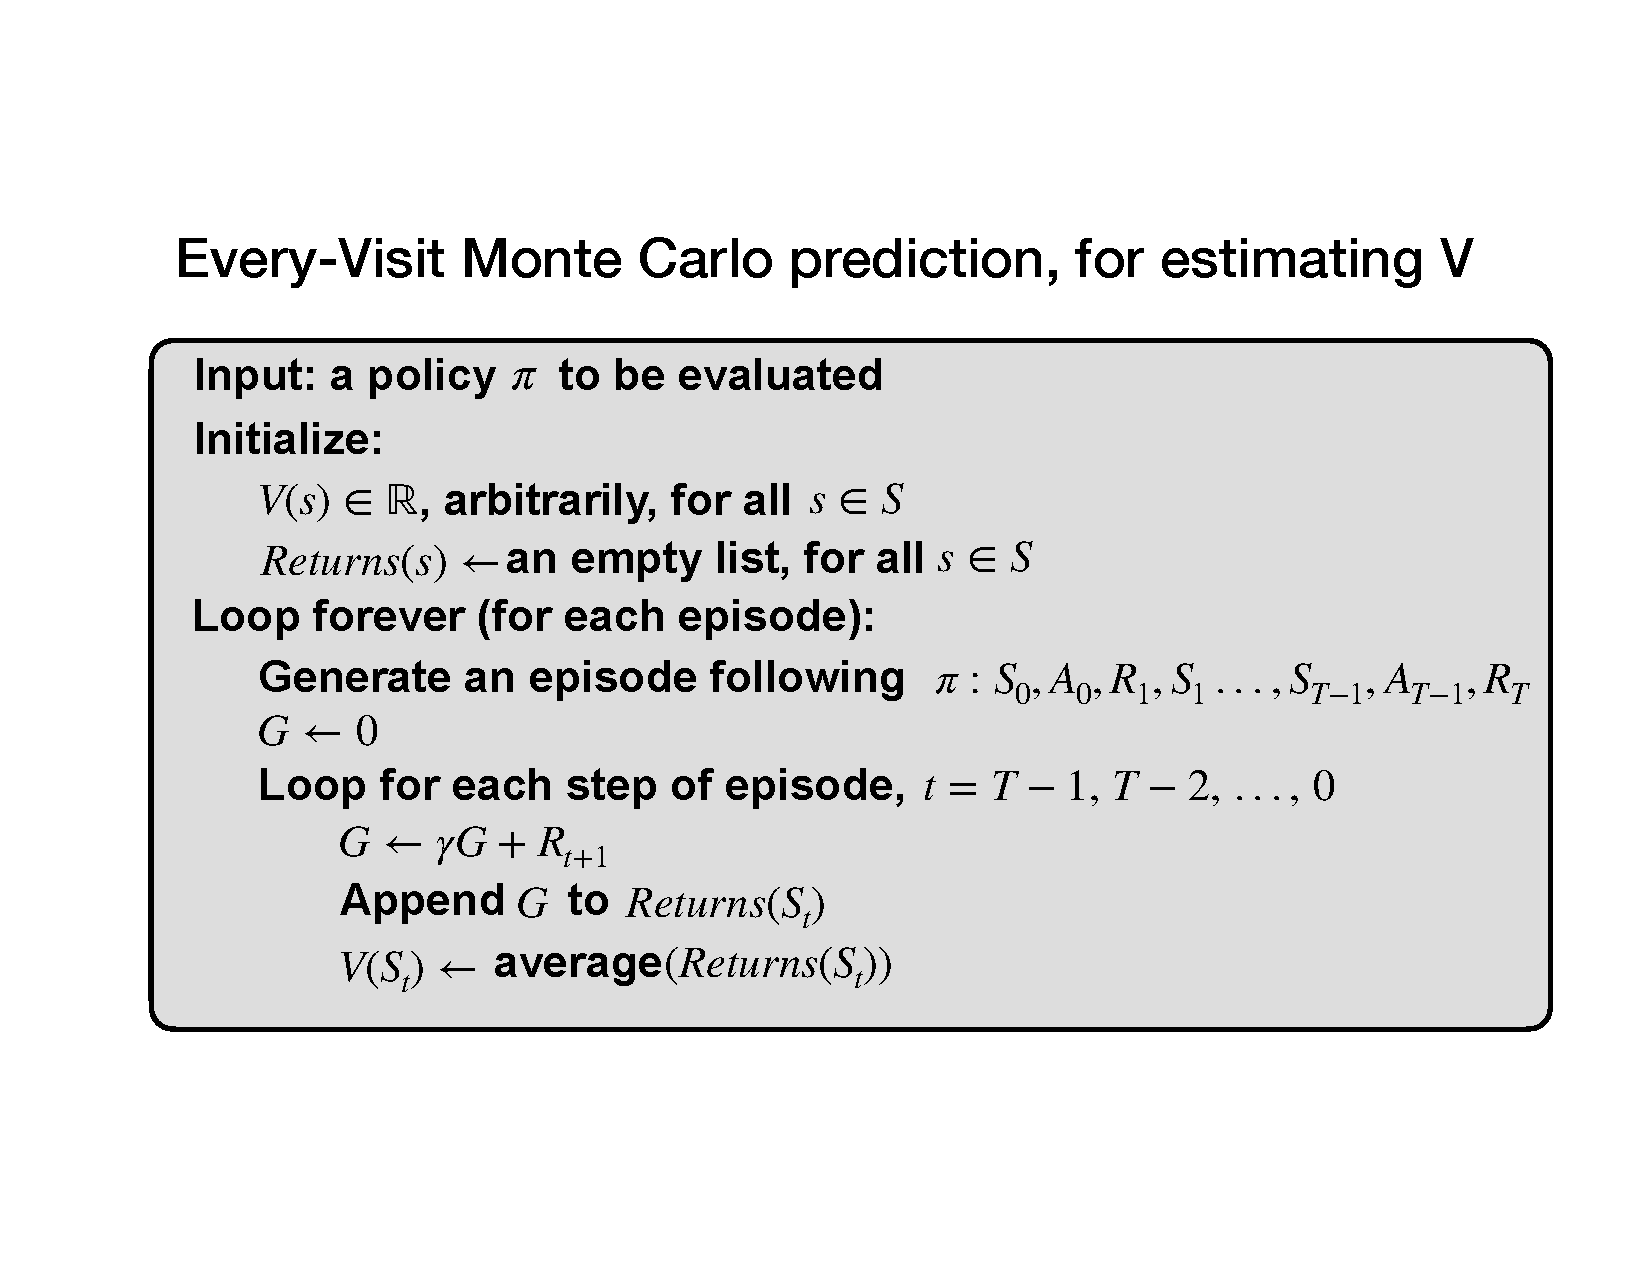
\includegraphics[width=0.8\linewidth]{figures/c2_mc_everyvisit.pdf}
\end{figure}

%%%%%%ANSWERS%%%%%%%5
% first-visit : 10
% every-visit : 10 + 9 + 8 + ... + 1 = (10)(11)/2 = 55

	\newpage
	\item 
In Policy Iteration, we used dynamic programming for the policy evaluation step, to compute $v_\pi$. 
Monte Carlo ES is a Generalized Policy Iteration (GPI) algorithm, that does not do a full policy evaluation step, before greedifying. How might you modify Monte Carlo ES, to do (more) complete policy evaluation steps before greedifying?

%% Old version, delete after November, 1, 2019
%
%Similar to dynamic programming, Monte Carlo estimates can be used
%for policy iteration. Although policy iteration can be used to 
%compute optimal policies, policy evaluation steps are only accurate 
%asymptotically for both dynamic programming and Monte Carlo methods.
%Generalized Policy Improvement (GPI), generalizes policy iteration without
%requiring exact policy evaluation steps. Explain what changes you would 
%make to value iteration (a dynamic programming GPI method) and 
%Monte Carlo with exploring starts to perform exact policy evaluation steps.
%
%%%%%%%ANSWERS%%%%%%5
%% MC ES:
%% Loop policy evaluation forever or until you know that the greedy policy will
%% never change. 
%% Remove previous estimates before every evaluation step
%% (not required if looping forever but will not change the process)
%
%% Value iteration
%% In policy evaluation step, apply the bellman equation over and over until
%% convergence as opposed to one pass over the state space.

	% MARTHAC: Update the figure in these questions
	%\item Consider the three state MDP below with terminal state $T_{3 }$ and $\gamma=1$.
Suppose you observe three episodes: $\{S_{0}, S_{1} , T_{3}\}$ with a return of 2, $\{S_{0}, S_{1} , T_{3}\}$ with a return of 2, $\{S_{0}, S_{2} , T_{3}\}$ with a return of 1.
What is the (every-visit) Monte-carlo estimator of the value for each of state $S_{0}, S_{1}, S_{2}$?
How would the Monte-Carlo estimates change if $r(S_{0}, A_{1}, S_{1}) = +1.00$?

\begin{figure}[h!]
  \center
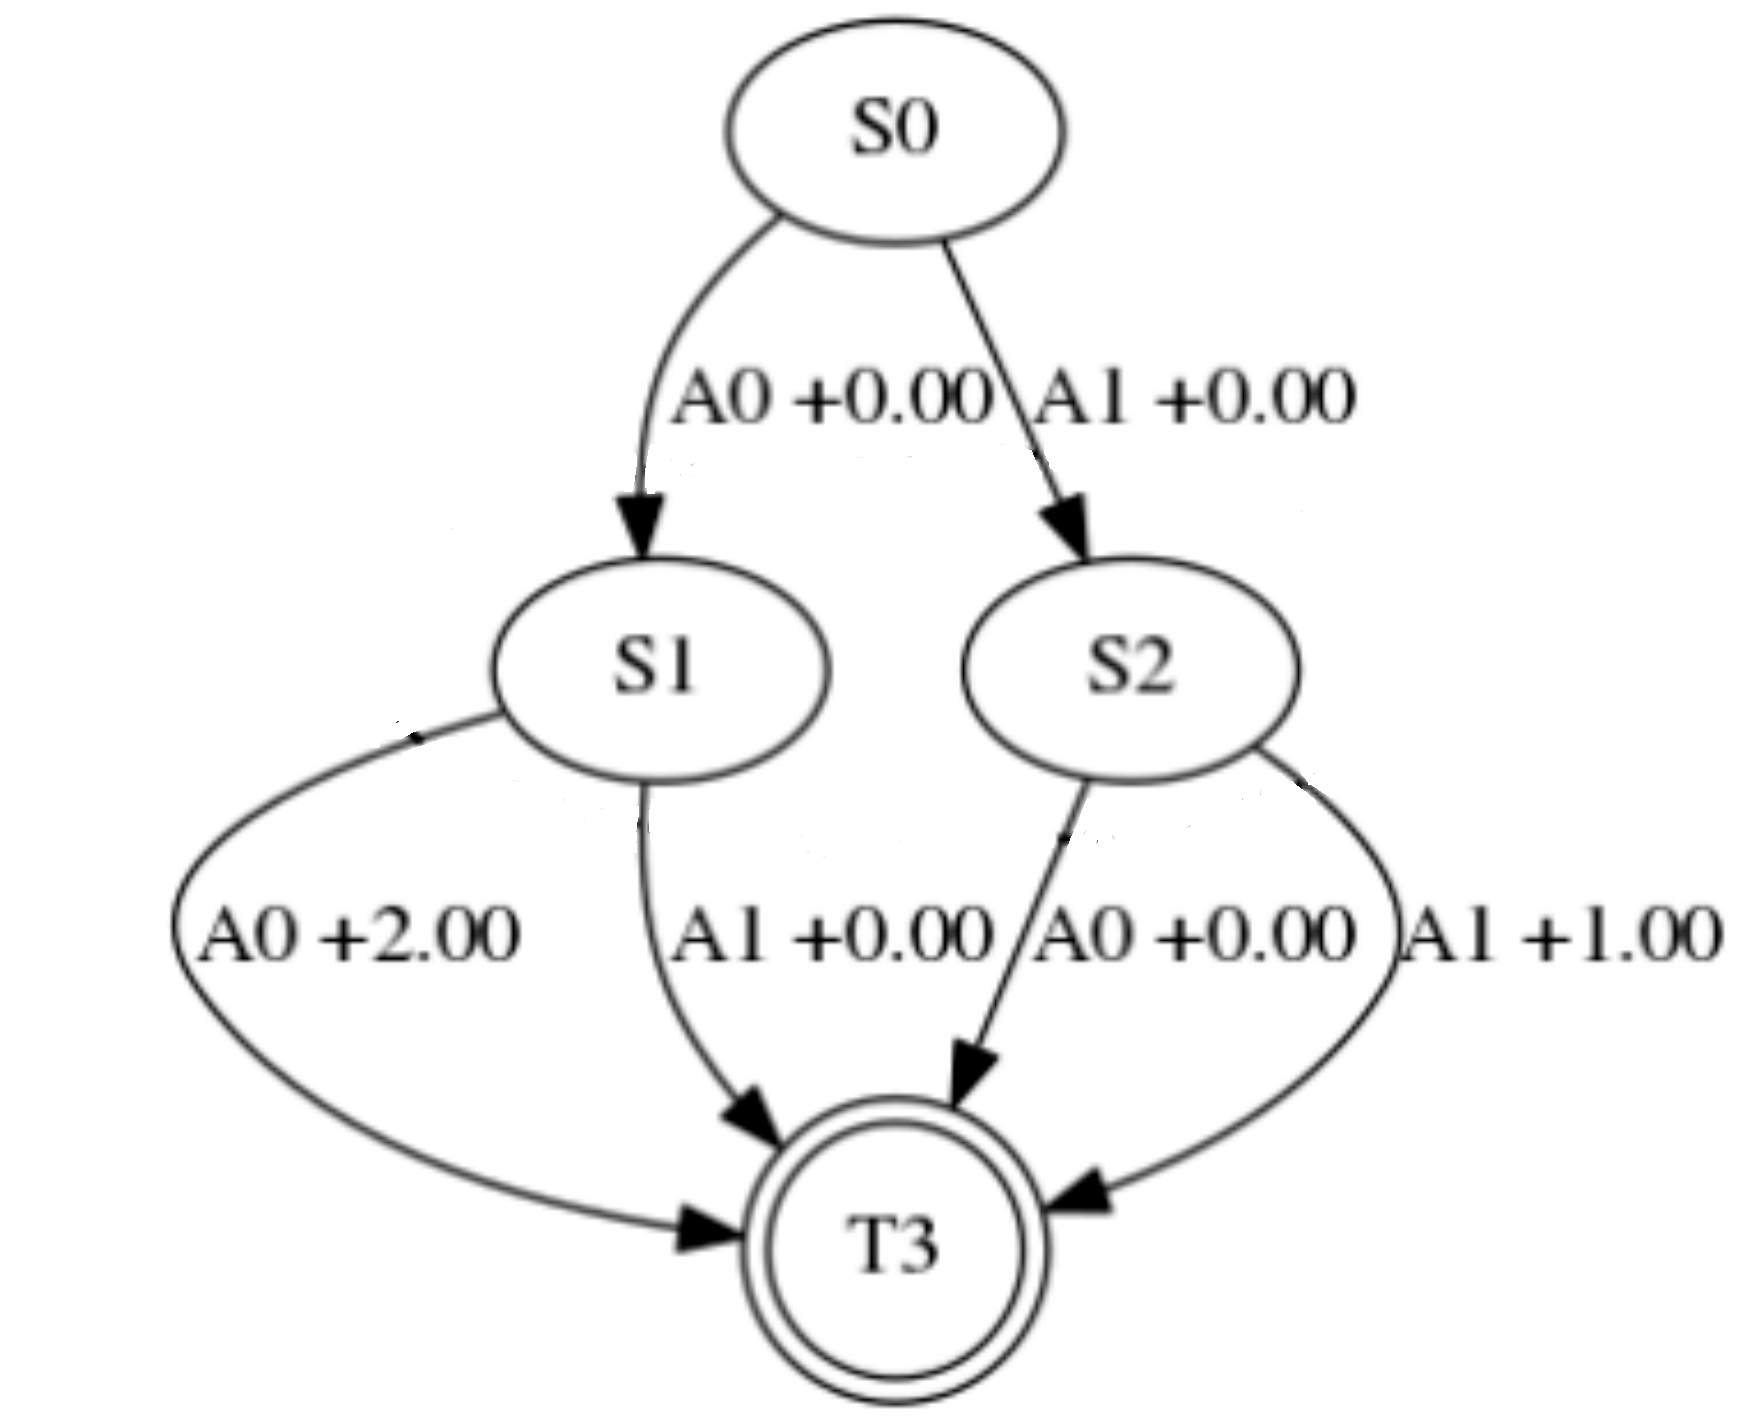
\includegraphics[width=0.5\linewidth]{figures/3state_edit.png}
\end{figure}
%%%%%%ANSWERS%%%%%%%5
% S_0 = 5/3
% S_1 = 2
% S_2 = 1
	%\item Consider the three state MDP from question $5$, but let $r(S_1, A_1,T_{3}) = +1.00$ and $r( S_{2}, A_{0},T_{3})=+2.00$.
You observe the following episodes:
$\{S_{0}, S_{1} , T_{3}\}$ with a return of 2, $\{S_{0}, S_{1} , T_{3}\}$ with a return of 2, $\{S_{0}, S_{1} , T_{3}\}$ with a return of 1, $\{S_{0}, S_{2} , T_{3}\}$ with a return of 1.
What is the (every-visit) Monte-carlo estimator of the value for each of state $S_{0}, S_{1}, S_{2}$?

%%%%%%ANSWERS%%%%%%%5
% S_0 = 6/4
% S_1 = 5/3
% S_2 = 1
	% MARTHAC: This question is sort of good practice, but is also confusing since you would never use IS for this; if I know my dice probabilities, then I'm just going to compute the expected value. A modification to a simple setting where it makes sense to use IS would be good
	%\item Suppose you would like to estimate the expected outcome for 
$3X^2$ where $X$ is the outcome of a fair die. 
You run an experiment and observe the following sequence of rolls
\[
	1,1,6,3,4.
\]
How would you use the above data to estimate the expected value 
$\mathbb{E}[3X^2]$ for a fair die if the above rolls where observed 
from a loaded die with $P(X=1) = 1/2$ and $P(X=i)=1/10$ for $i=2,3,4,5,6$?


%%% ANSWERS %%%%%
%   0.1666/0.5*(1+1) + 0.1666/0.1*(6^2+3^2+4^2) = 102.333 => estimate = 61.4


	\item Off-policy Monte Carlo prediction allows us to use sample trajectories to 
estimate the value function for a policy that may be different than the one
used to generate the data. Consider the following MDP, with two states $B$ and $C$, with 1 action in state $B$ and two actions in state $C$, with $\gamma = 1.0$. In state $C$ both actions transition to the terminating state with $A=1$ following the blue path to receive a reward $R=1$ and $A=2$ following the green path to receive a reward $R=10$. Assume the target policy $\pi$ has $\pi(A = 1 | C) = 0.9$ and $\pi(A = 2 | C) = 0.1$, and that the behaviour policy $b$ has $b(A = 1 | C) = 0.25$ and $b(A = 2 | C) = 0.75$.
\begin{enumerate}
\item What are the true values $v_\pi$?
\item Imagine you got to execute $\pi$ in the environment for one episode, and observed the episode trajectory $S_0 = B, A_0 = 1, R_1 = 1, S_1 = C, A_1 = 1, R_2 = 1$. What is the return for $B$ for this episode? Additionally, what are the value estimates $V_\pi$, using this one episode with Monte Carlo updates?
\item But, you do not actually get to execute $\pi$; the agent follows the behaviour policy $b$. Instead, you get one episode when following $b$, and observed the episode trajectory $S_0 = B, A_0 = 1, R_1 = 1, S_1 = C, A_1 = 2, R_2 = 10$. What is the return for $B$ for this episode? Notice that this is a return for the behaviour policy, and using it with Monte Carlo updates (without importance sampling ratios) would give you value estimates for $b$.  
\item But, we do not actually want to estimate the values for behaviour $b$, we want to estimates the values for $\pi$. So, we need to use importance sampling ratios for this return. What is the return for $B$ using this episode, but now with importance sampling ratios? Additionally, what is the resulting value estimate for $V_\pi$ using this return? 
\end{enumerate}
\begin{figure}[h!]
  \center
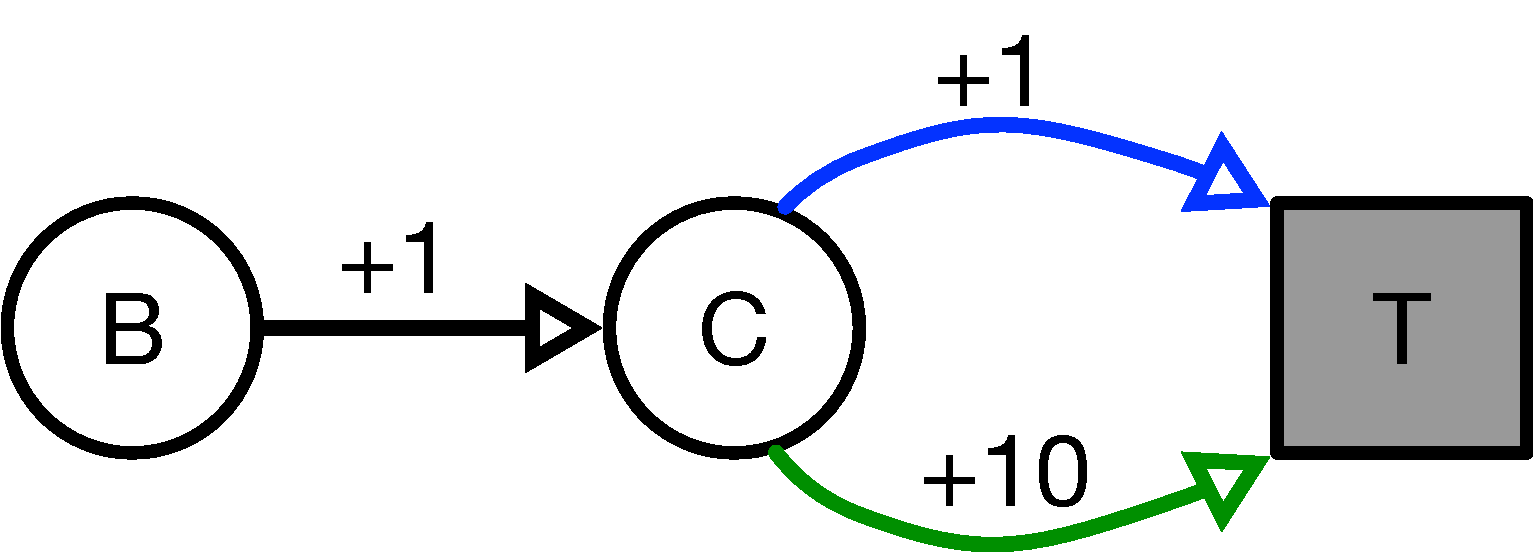
\includegraphics[width=0.5\linewidth]{figures/c2_2state.pdf}
\end{figure}

%%%%%%ANSWERS%%%%%%
% (a) vpi(C) = 1.9, vpi(B) = 2.9
% (b) Return is 2
% (c) Return is 11
% (d) Return is 1.47



	\item Let $\rho_{t} = \frac{\pi(A_{t} | S_{t})}{b(A_{t} | S_{t})}$.
\begin{enumerate}
    \item Verify that $\mathbb{E}_{b}[\rho_{t} | S_t=s] = 1$.
    \item Verify that $\mathbb{E}_{b}[\rho_{t} R_{t+1} | S_t = s] = \mathbb{E}_{\pi}[R_{t+1} | S_t = s]$.
    \item What is the variance of the importance corrected one-step reward, $\mathbb{V}(\rho_{t} R_{t+1} | S_t =s)$? When would this variance be large?
\end{enumerate}
\end{enumerate}

\end{document}

%%% Local Variables:
%%% mode: latex
%%% TeX-master: t
%%% End:
